%%%%%%%%%%%%%%%%%%%%%%%%%%%%%%%%%%%%%%%%%%%%%%%%%%%%%%%%%%%%%%%%%%%%%%%%
% Plantilla TFG/TFM
% Escuela Politécnica Superior de la Universidad de Alicante
% Realizado por: Jose Manuel Requena Plens
% Contacto: info@jmrplens.com / Telegram:@jmrplens
%%%%%%%%%%%%%%%%%%%%%%%%%%%%%%%%%%%%%%%%%%%%%%%%%%%%%%%%%%%%%%%%%%%%%%%%

\chapter{Human Body Prediction Results}\label{chap:results}

In this chapter we will go through the results obtained from the experiments
performed in the previous chapter. We will start by evaluating the predictive
performance of our model, followed by a discussion of the results of generated
bodies and their implications.

\section{Evaluation}

\begin{figure}
	\centering
	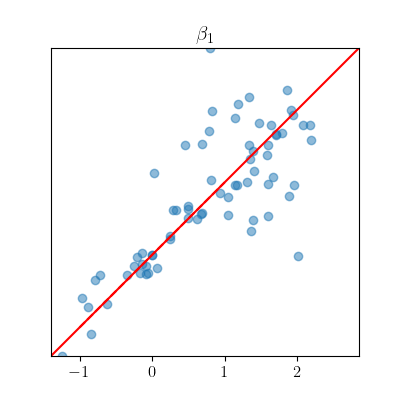
\includegraphics[width=0.3\textwidth]{files/predictions_beta/beta_1.png}
	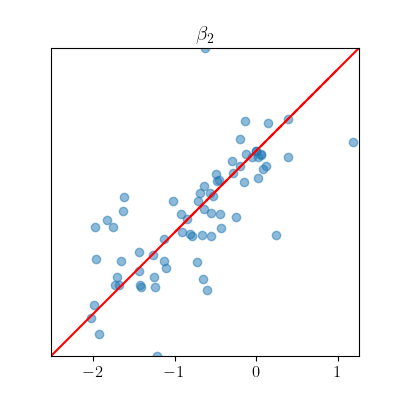
\includegraphics[width=0.3\textwidth]{files/predictions_beta/beta_2.png}
	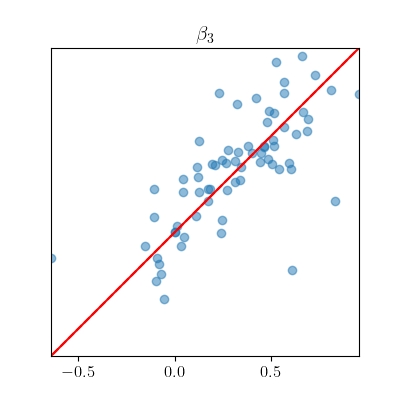
\includegraphics[width=0.3\textwidth]{files/predictions_beta/beta_3.png}
	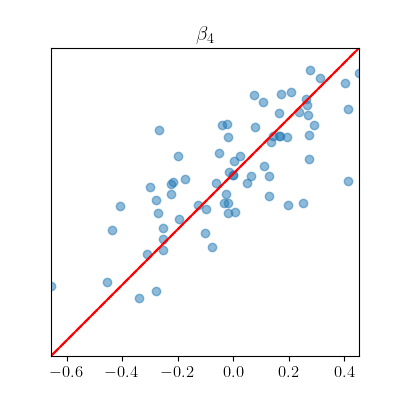
\includegraphics[width=0.3\textwidth]{files/predictions_beta/beta_4.png}
	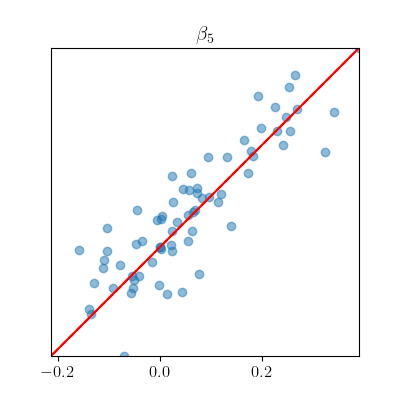
\includegraphics[width=0.3\textwidth]{files/predictions_beta/beta_5.png}
	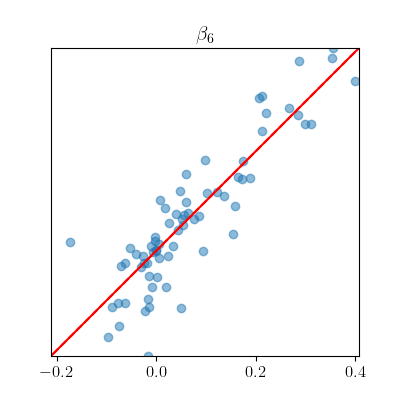
\includegraphics[width=0.3\textwidth]{files/predictions_beta/beta_6.png}
	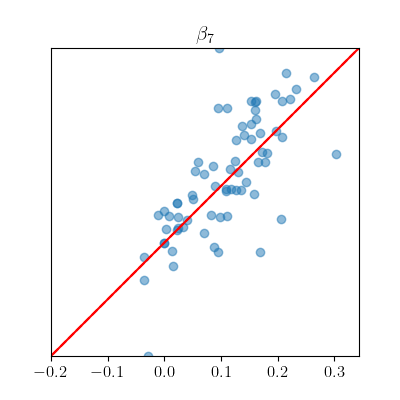
\includegraphics[width=0.3\textwidth]{files/predictions_beta/beta_7.png}
	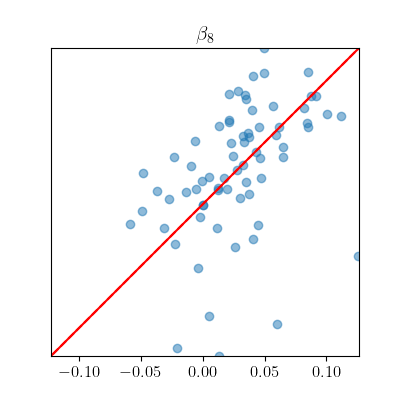
\includegraphics[width=0.3\textwidth]{files/predictions_beta/beta_8.png}
	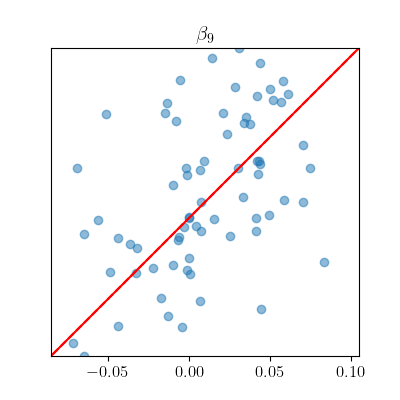
\includegraphics[width=0.3\textwidth]{files/predictions_beta/beta_9.png}
	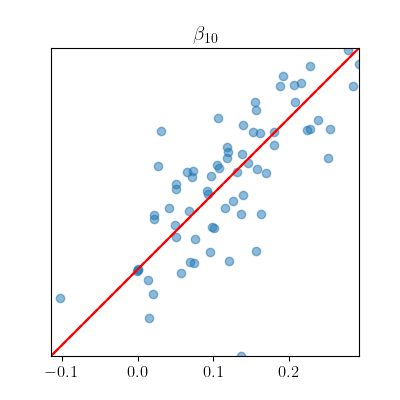
\includegraphics[width=0.3\textwidth]{files/predictions_beta/beta_10.png}
	\caption[Predictions vs ground truth]{Predictions (y-axis) vs ground truth (x-axis) for each $\beta$ parameter.}
	\label{fig:scatter}
\end{figure}

\subsection{Quantitative results}

The mean \gls{mae} of the model in the test set when predicting the $\beta$
parameter is \textbf{0.064}. Figure \ref{fig:scatter} shows the predictions of
the model vs the ground truth, and Figure \ref{fig:fold-mae} shows the
\gls{mae} for each $\beta$ per fold. We can see that the model is able to
predict the correct value in most cases, but it has some problems with
outliers.

\begin{figure}[H]
	\centering
	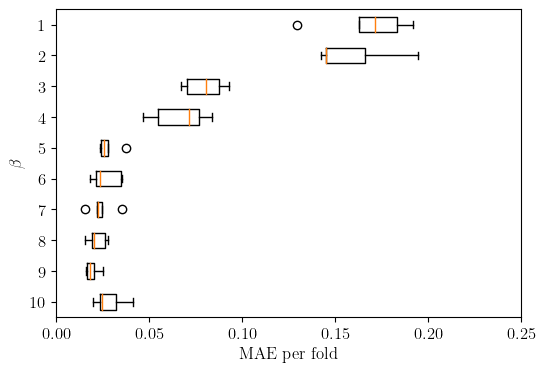
\includegraphics[width=300pt]{files/mae_folds.png}
	\caption{MAE for each $\beta$ per fold.}
	\label{fig:fold-mae}
\end{figure}

\begin{figure}[H]
	\centering
	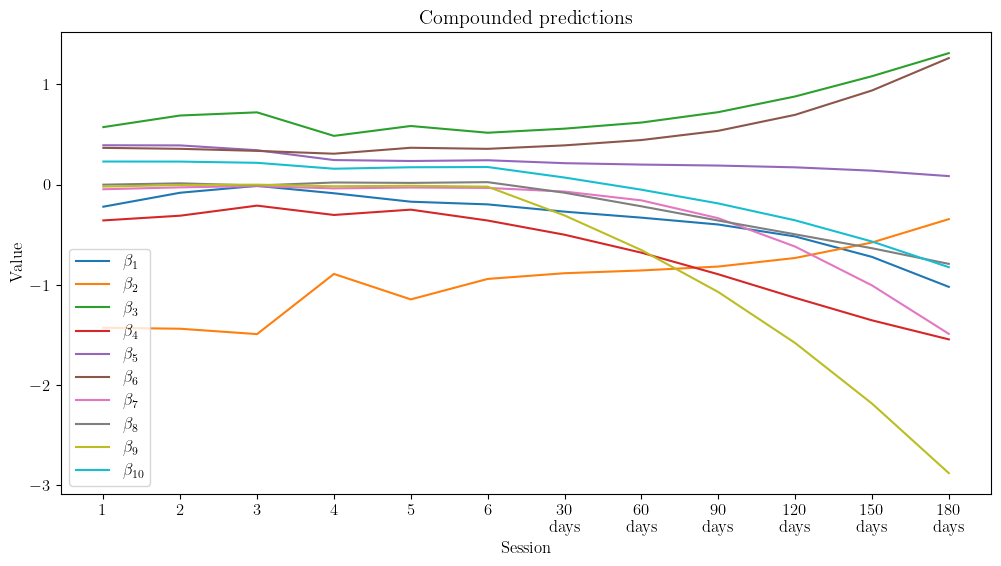
\includegraphics[width=\textwidth]{files/compounded.png}
	\caption{Compounded predictions for 180 days.}
	\label{fig:compounded}
\end{figure}

However, Figure \ref{fig:compounded} shows that the model's predictions begin
to diverge once we try to feed the predictions back into the model. This makes
it unsuitable for long-term predictions without some form of regularization.

One possible explanation is that we are trying to predict more into the future
than the timescale of our scans. We believe that obtaining more scans would
help the model to learn the long-term dynamics of the patient.

\subsection{Qualitative results}

Although it is hard to evaluate the quality of the generated bodies, we can see
that the model is able to generate bodies that look like the patient's body.
Figure {\ref{fig:pred-1}} shows that the predicted bodies after 30 days look
plausible.

As we saw in the previous chapter, Figure \ref{fig:predicted-betas} shows that
the value for $\beta_2$, inversely correlated with \gls{bmi}, tends to
increase, so the predicted bodies tend to be thinner.

In spite of this, the model is unstable if we try to use the predictions as
input for the next prediction. Figure \ref{fig:compounded} shows that the
predicted values for the $\beta$ parameter diverge. However, if we take a look
at the predicted bodies, in Figure {\ref{fig:pred-2}} we can see that the
predicted bodies still look plausible.

\begin{figure}[h]
	\centering
	\begin{subfigure}{\textwidth}
		\centering
		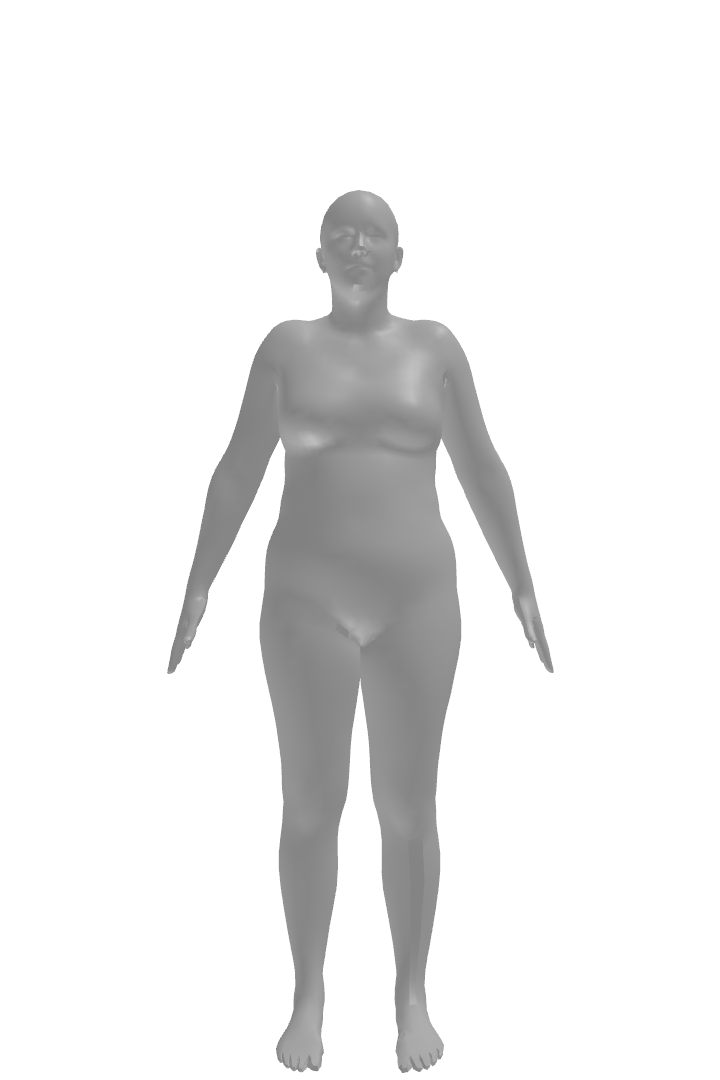
\includegraphics[width=60pt]{files/patients/9_2}
		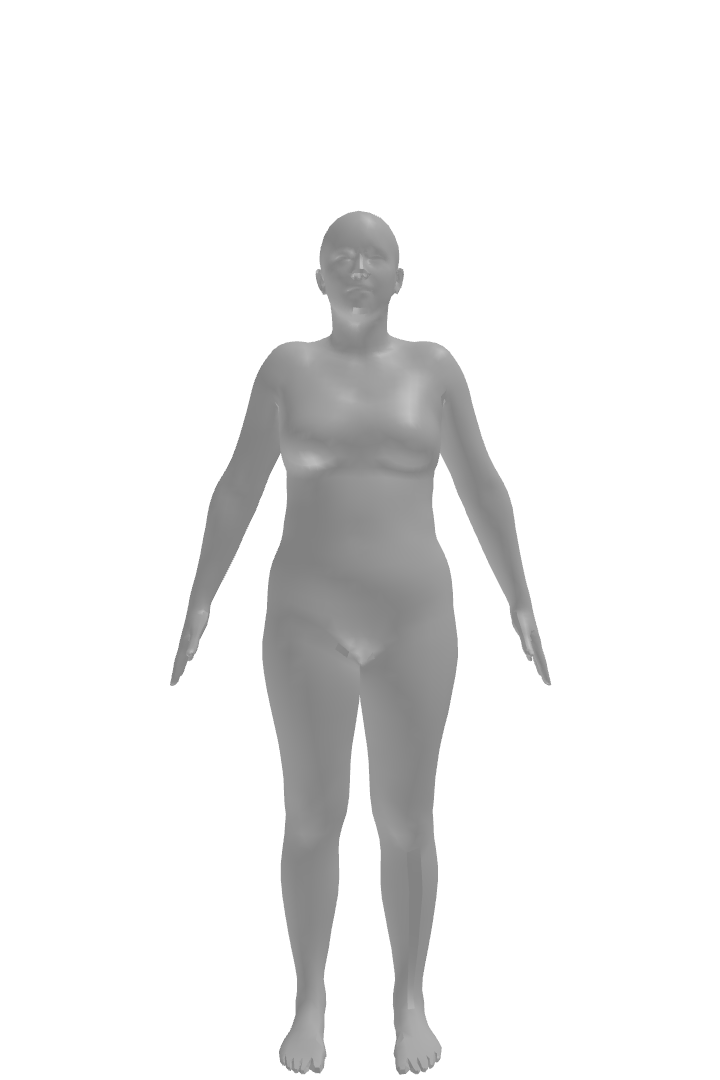
\includegraphics[width=60pt]{files/patients/9_3}
		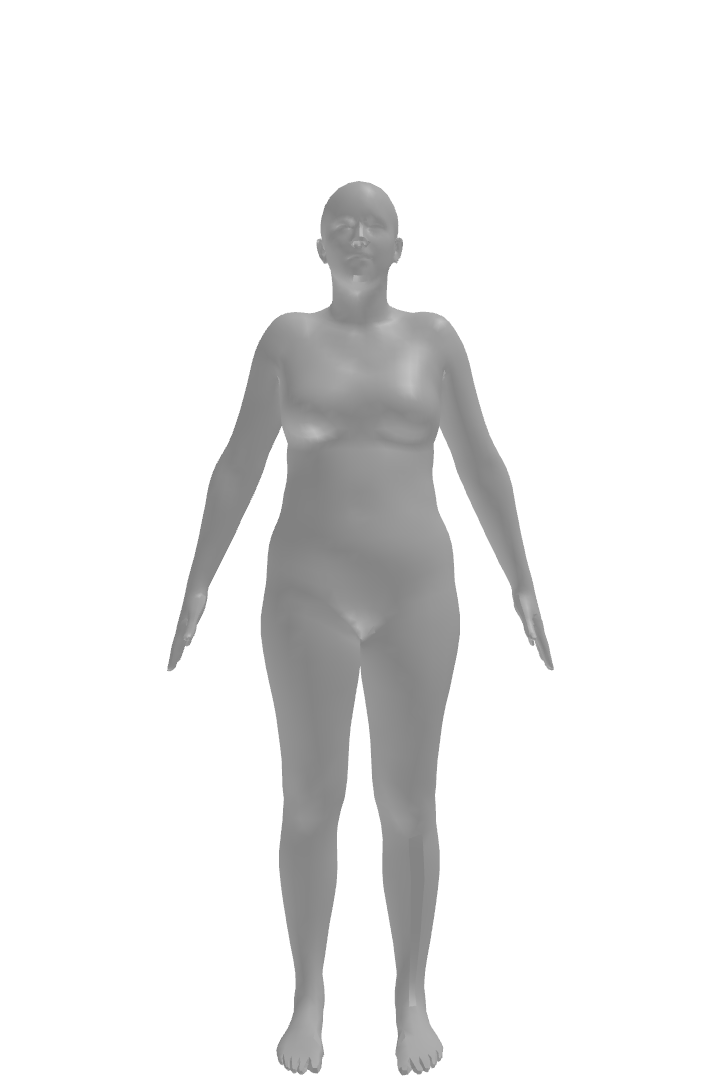
\includegraphics[width=60pt]{files/patients/9_4}
		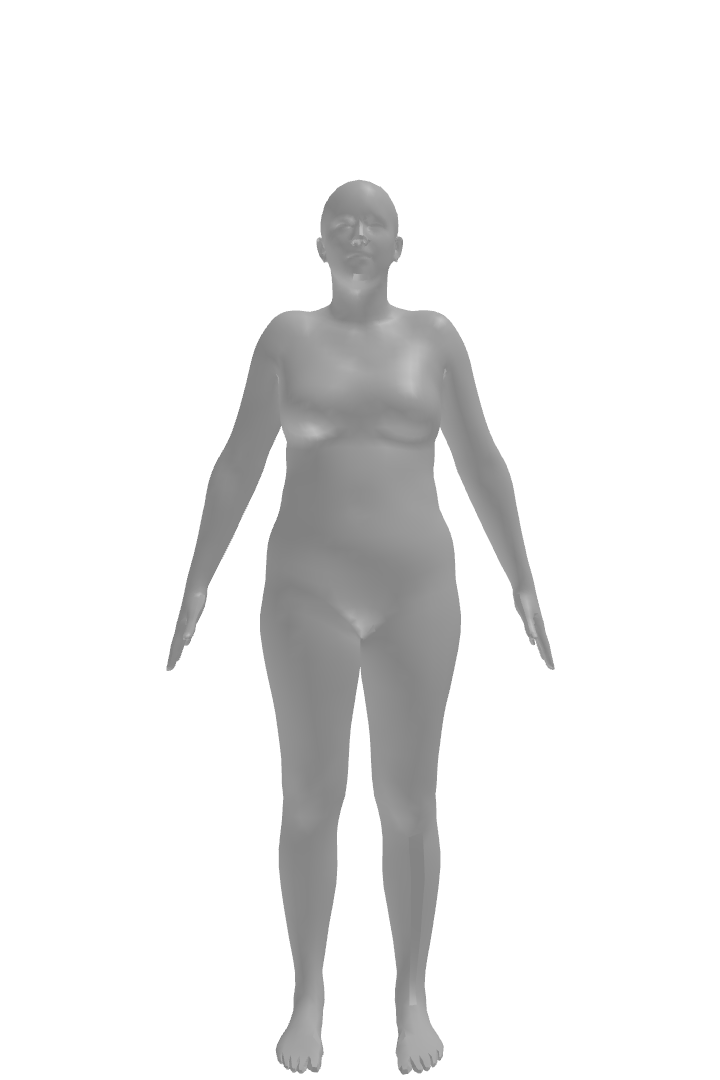
\includegraphics[width=60pt]{files/patients/9_5}
		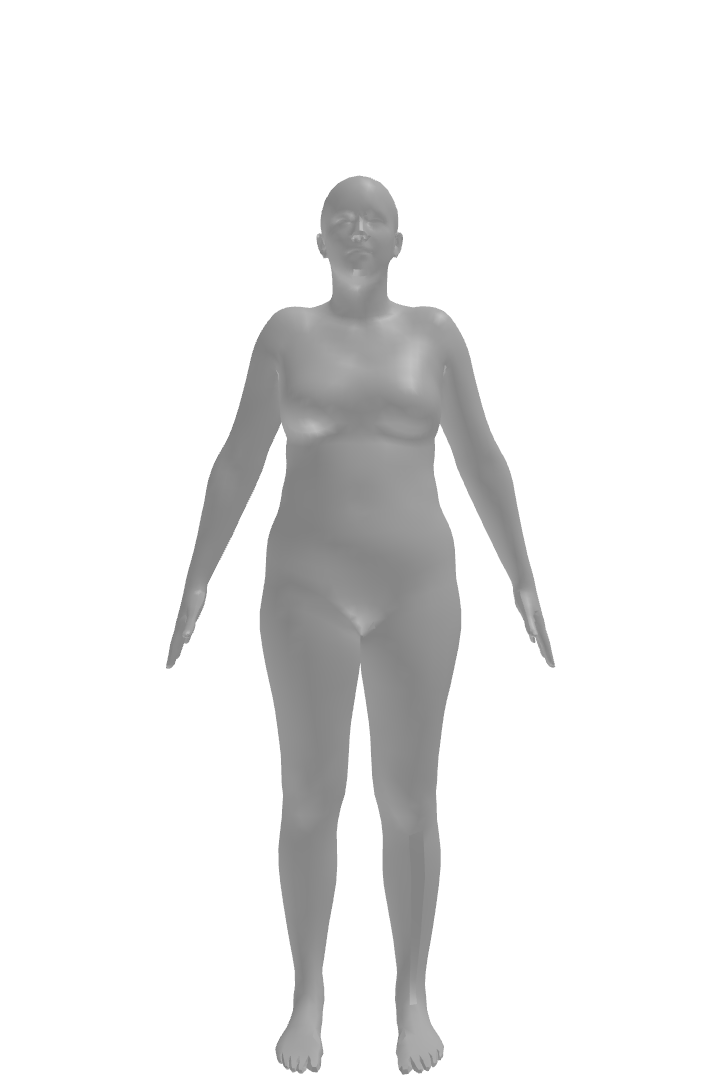
\includegraphics[width=60pt]{files/patients/9_6}
		\hspace{10pt}
		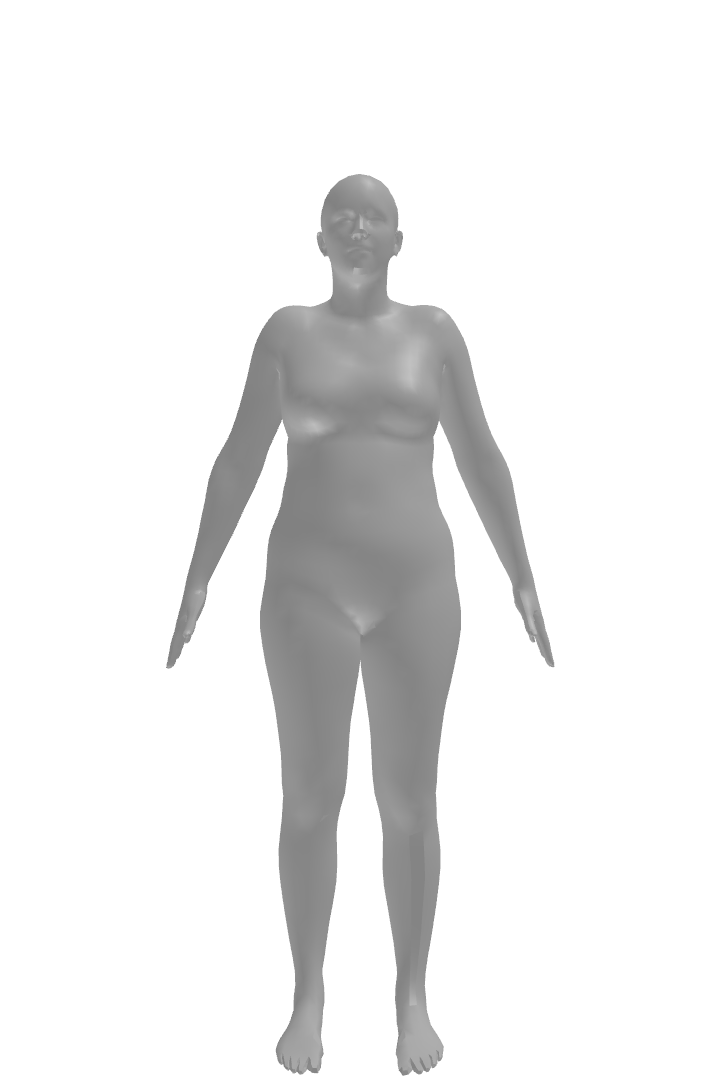
\includegraphics[width=60pt]{files/patients/9_predicted}
	\end{subfigure}
	\linebreak
	\begin{subfigure}{\textwidth}
		\centering
		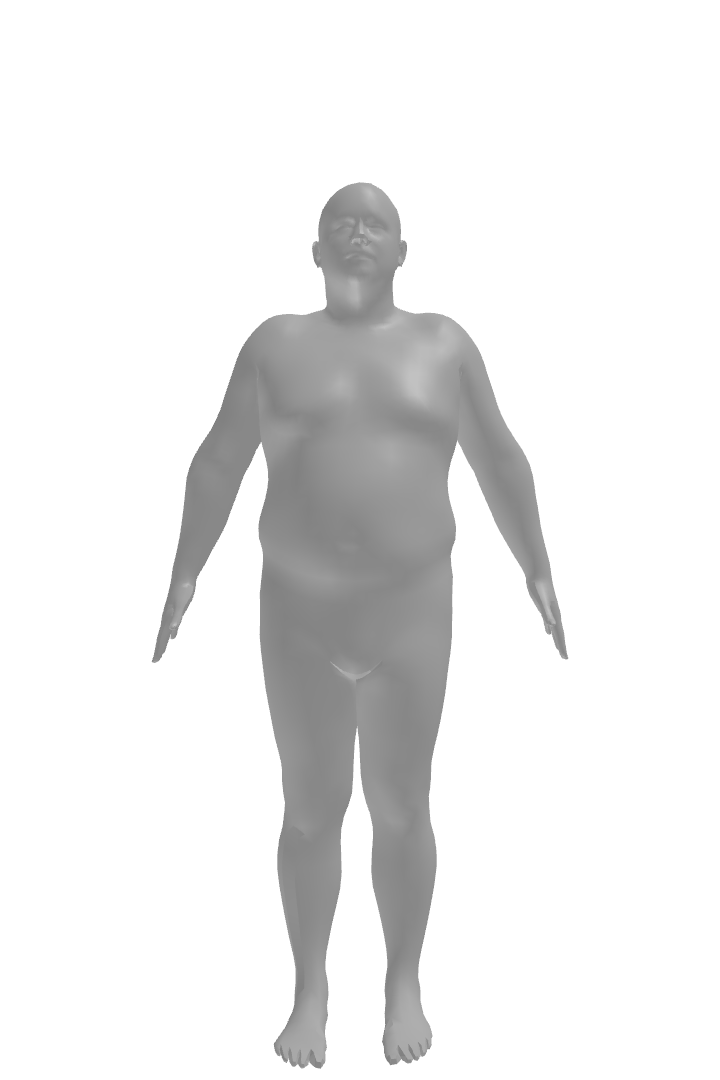
\includegraphics[width=60pt]{files/patients/128_1}
		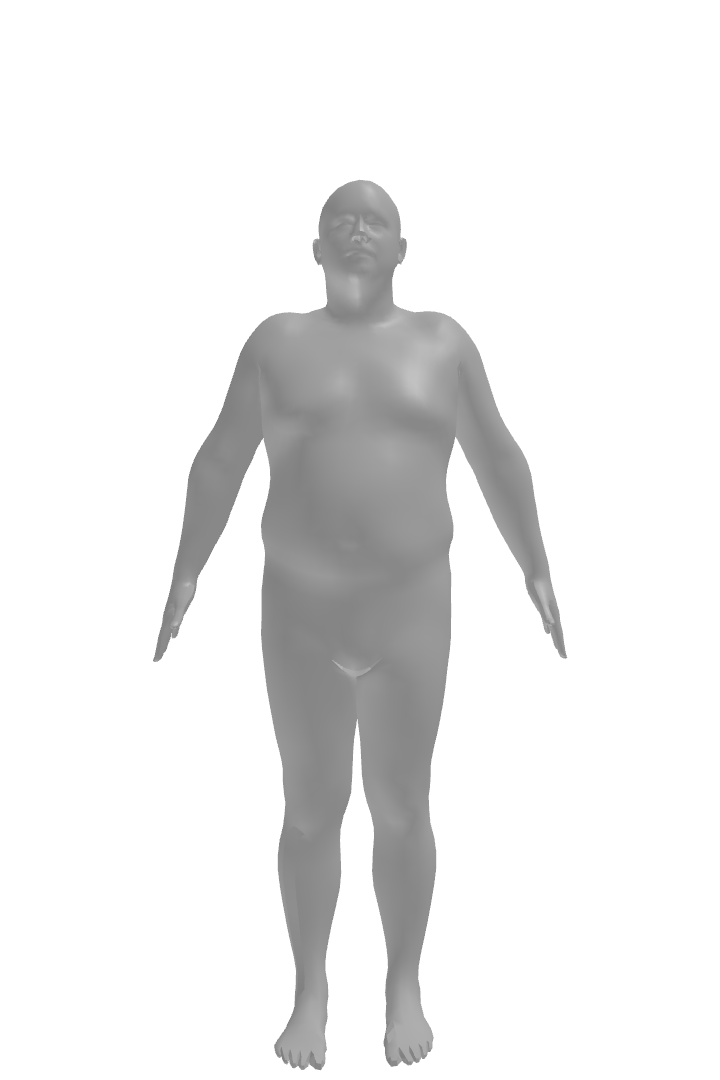
\includegraphics[width=60pt]{files/patients/128_2}
		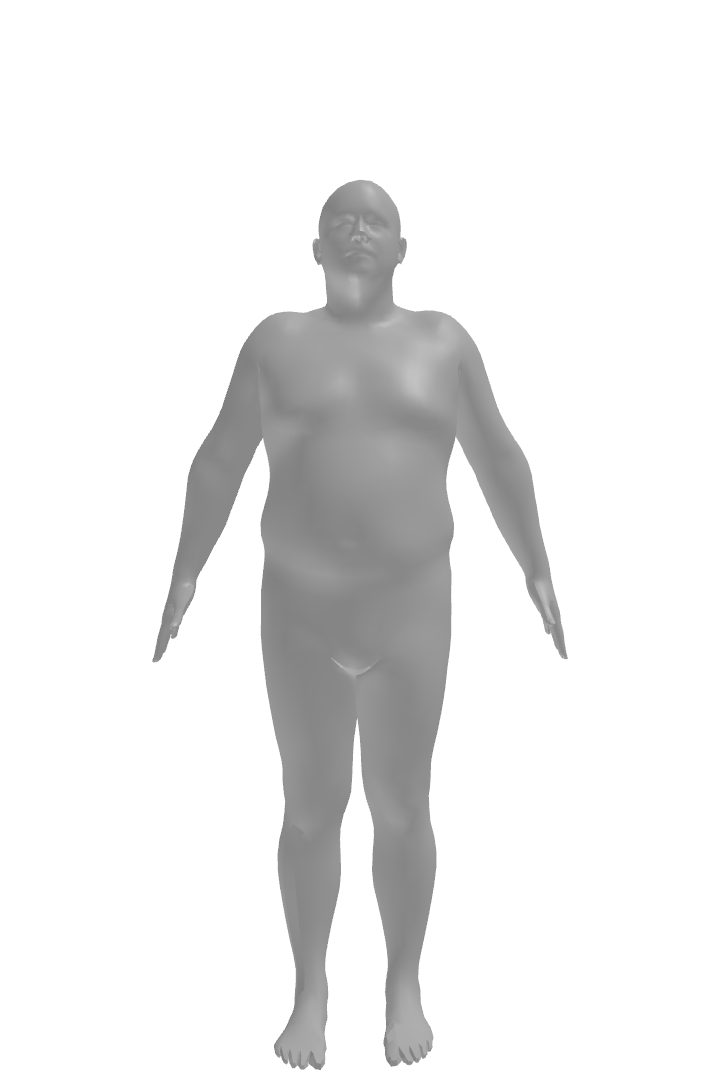
\includegraphics[width=60pt]{files/patients/128_3}
		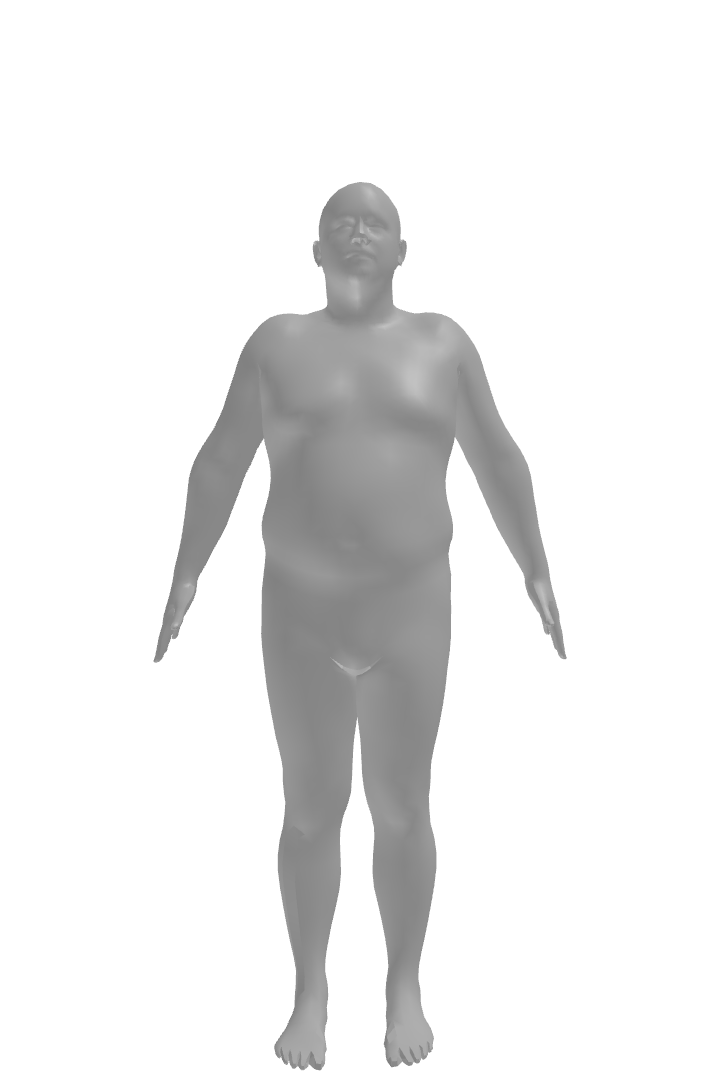
\includegraphics[width=60pt]{files/patients/128_4}
		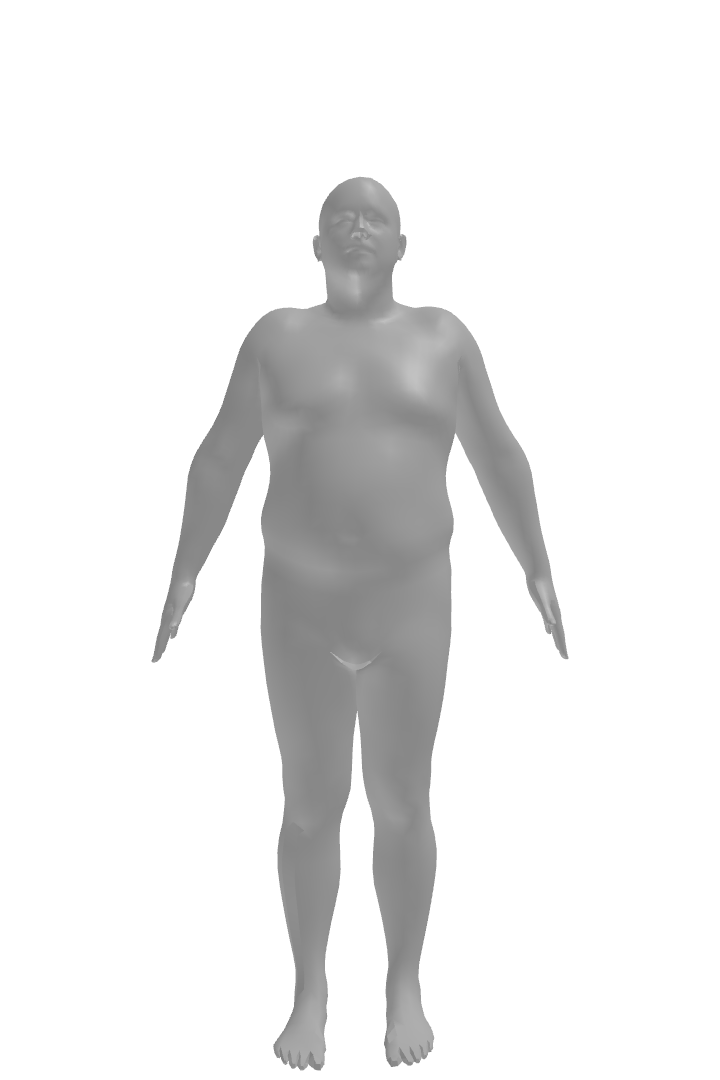
\includegraphics[width=60pt]{files/patients/128_5}
		\hspace{10pt}
		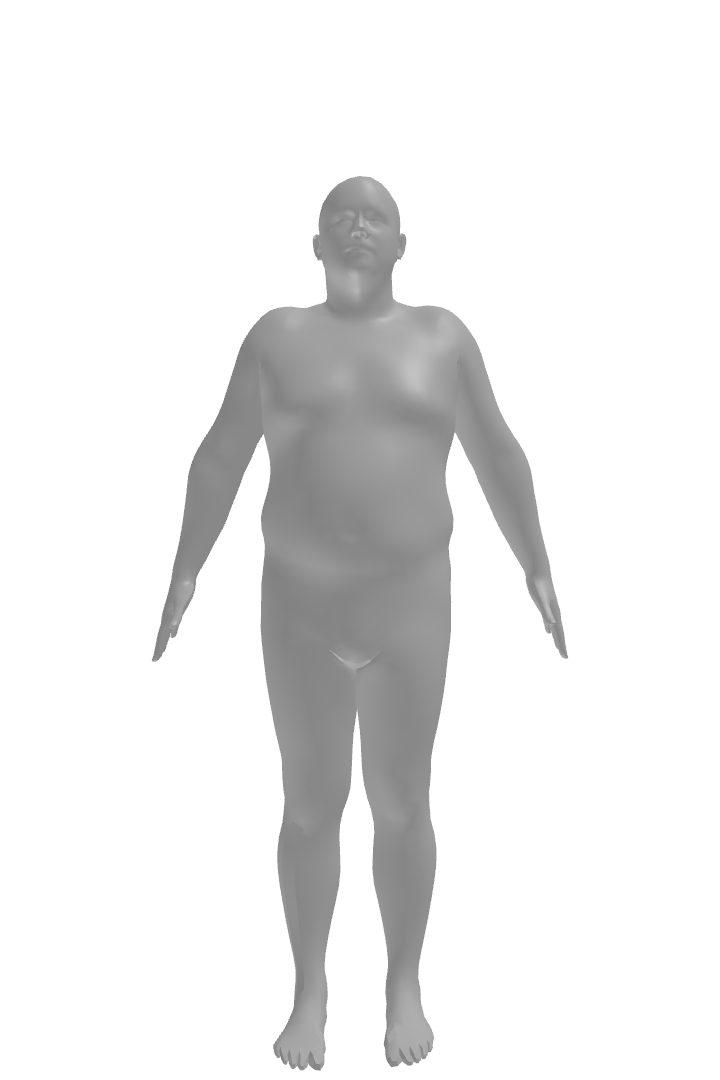
\includegraphics[width=60pt]{files/patients/128_predicted}
	\end{subfigure}
	\caption{Predicted bodies for two patients.}
	\label{fig:pred-1}
\end{figure}

\begin{figure}[h]
	\centering
	\begin{subfigure}{0.3\textwidth}
		\centering
		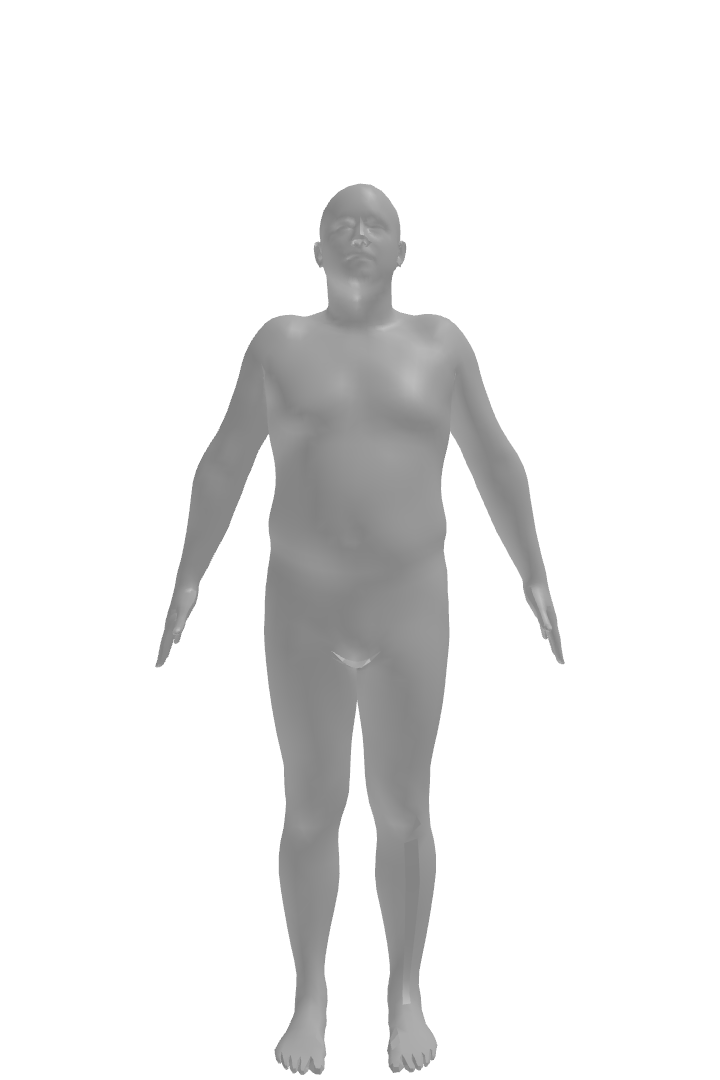
\includegraphics[width=120pt]{files/patients/2_predicted_2.png}
		\caption{93.8 kg}
	\end{subfigure}
	\begin{subfigure}{0.3\textwidth}
		\centering
		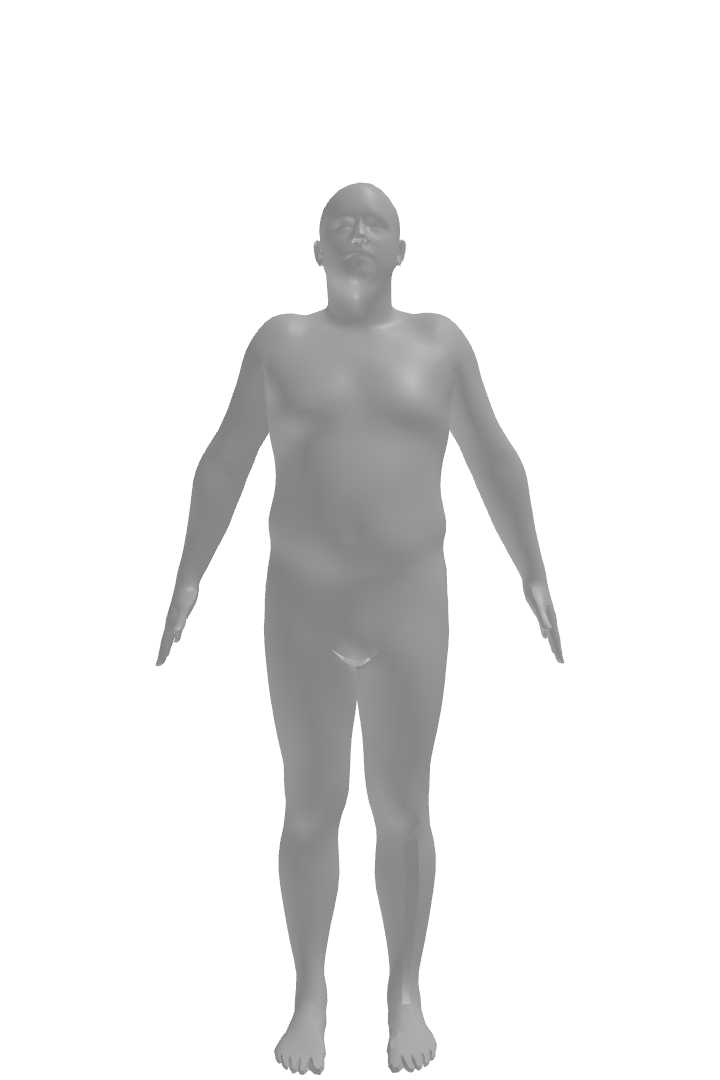
\includegraphics[width=120pt]{files/patients/2_predicted_3.png}
		\caption{93.1 kg}
	\end{subfigure}
	\begin{subfigure}{0.3\textwidth}
		\centering
		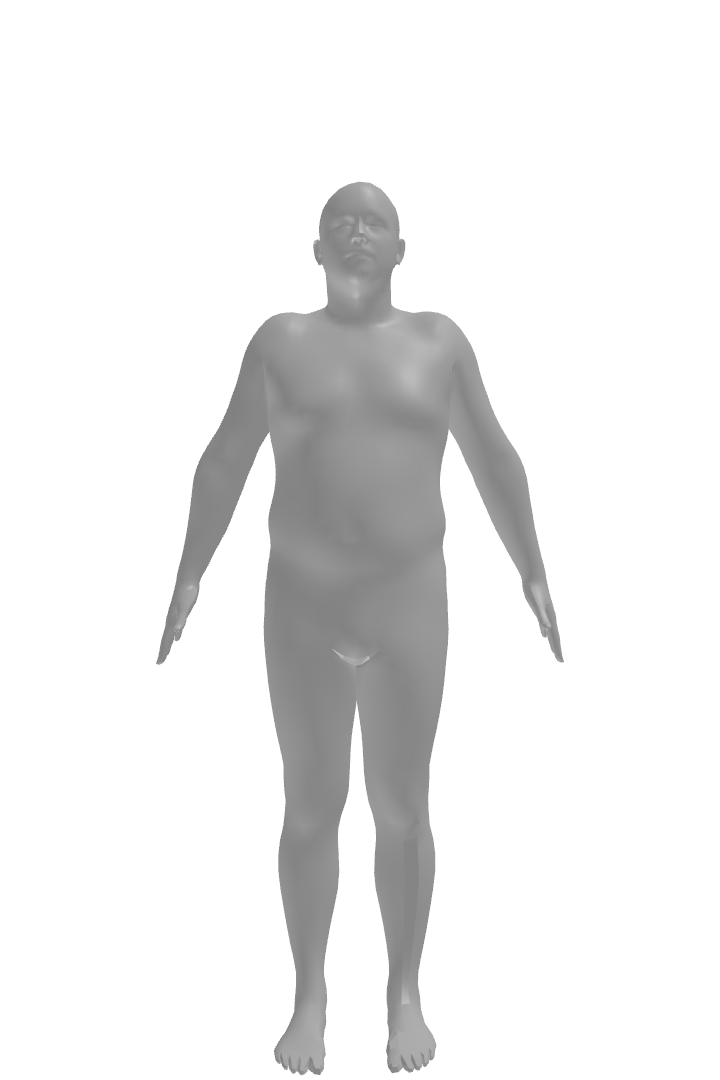
\includegraphics[width=120pt]{files/patients/2_predicted_4.png}
		\caption{92.4 kg}
	\end{subfigure}
	\begin{subfigure}{0.3\textwidth}
		\centering
		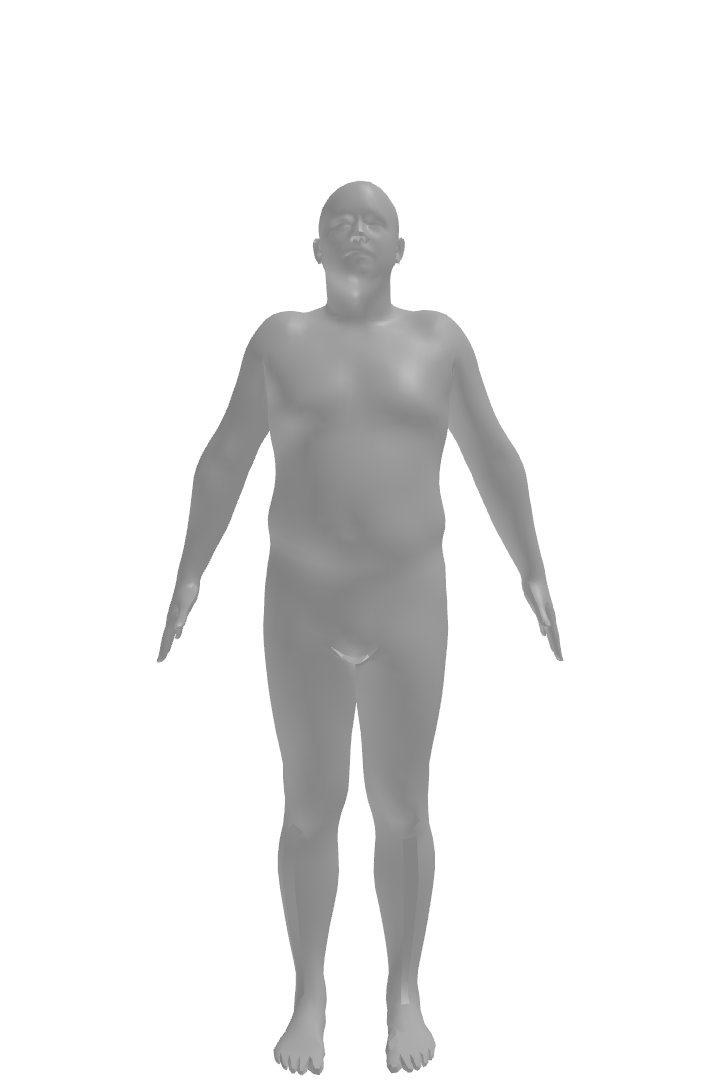
\includegraphics[width=120pt]{files/patients/2_predicted_5.png}
		\caption{91.6 kg}
	\end{subfigure}
	\begin{subfigure}{0.3\textwidth}
		\centering
		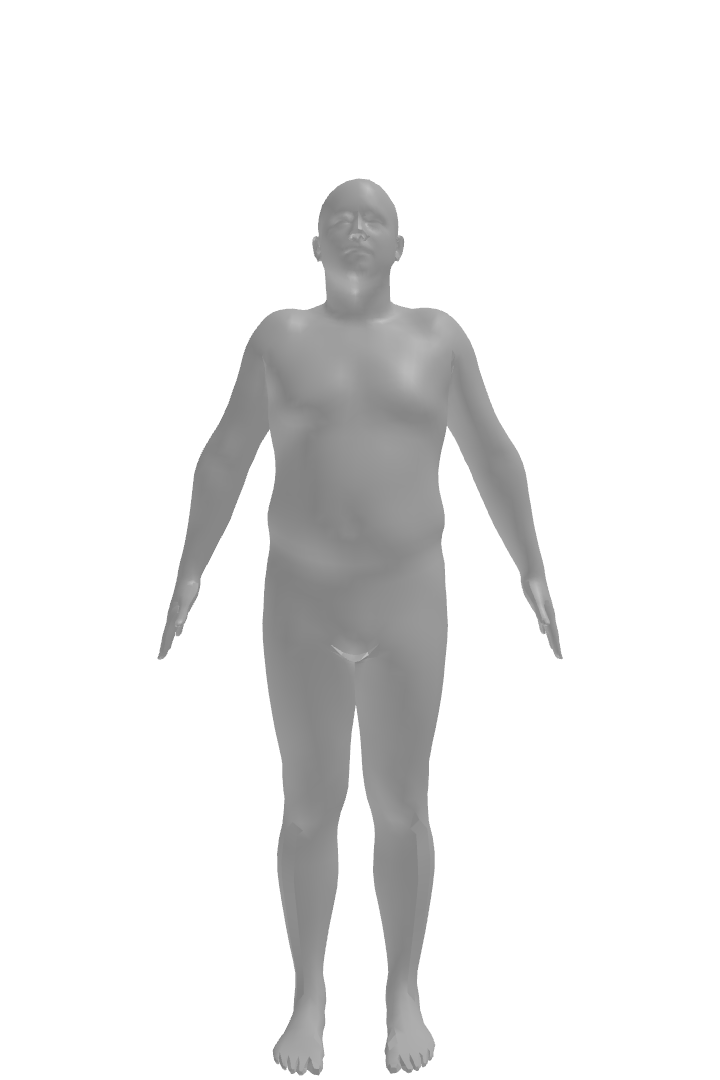
\includegraphics[width=120pt]{files/patients/2_predicted_6.png}
		\caption{90.8 kg}
	\end{subfigure}
	\begin{subfigure}{0.3\textwidth}
		\centering
		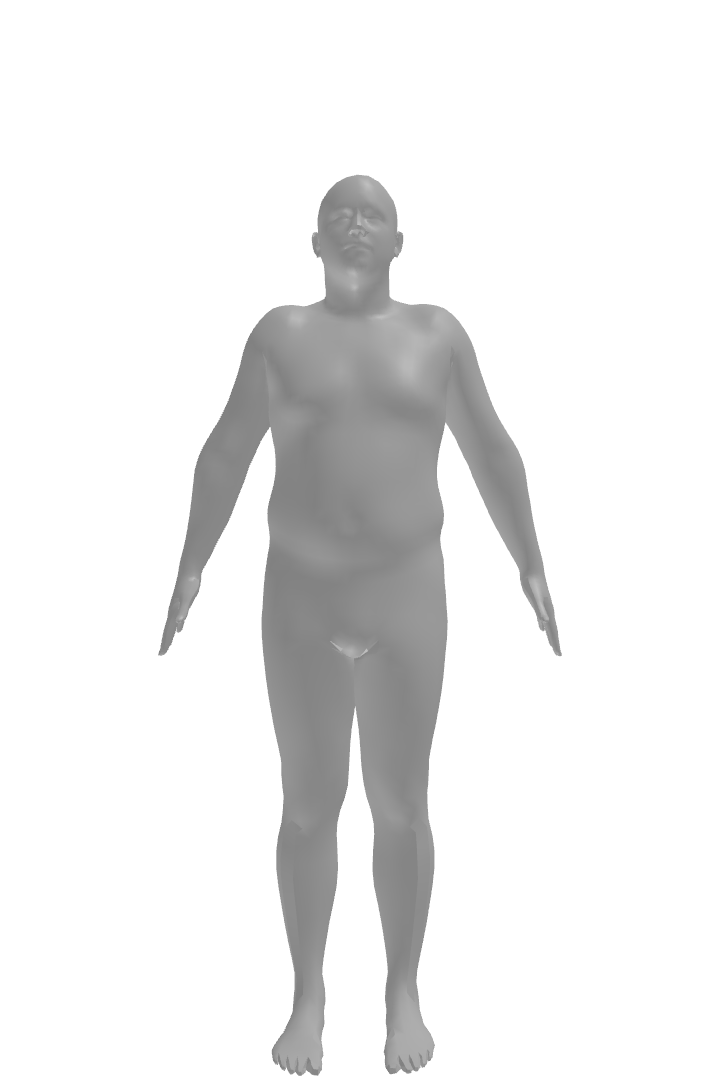
\includegraphics[width=120pt]{files/patients/2_predicted_7.png}
		\caption{90.0 kg}
	\end{subfigure}
	\caption[Compounded generations]{Compounded generations for a patient after 30, 60, 90, 120, 150, and 180 days.}
	\label{fig:pred-2}
\end{figure}

\section{Discussion}

\begin{figure}[h]
	\centering
	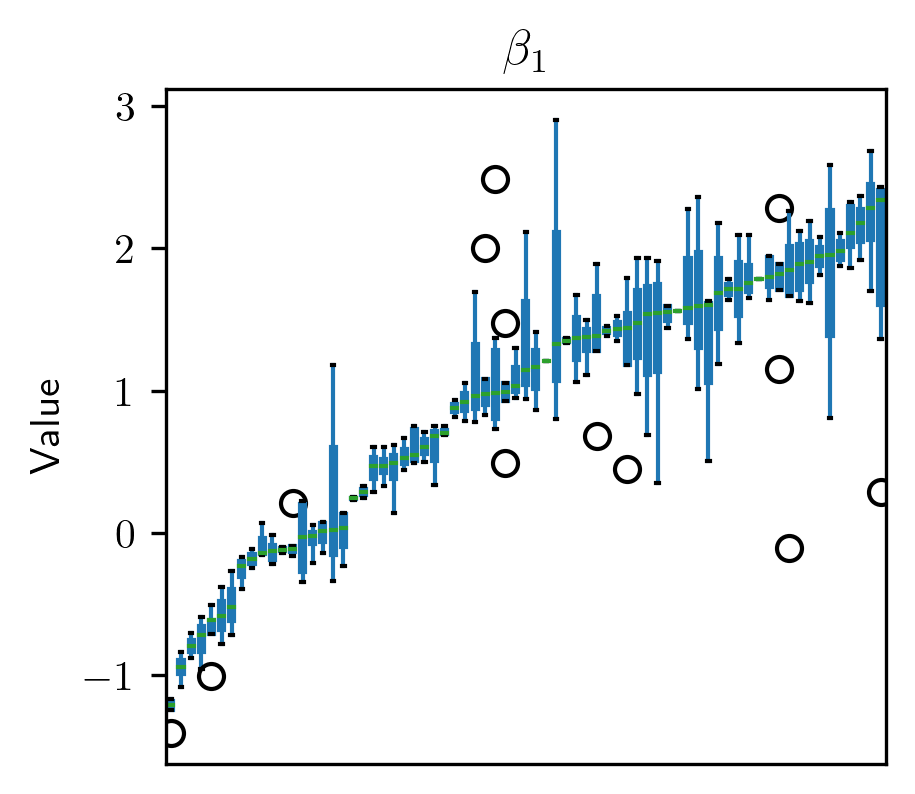
\includegraphics[width=0.3\textwidth]{files/beta_var/beta_1_var.png}
	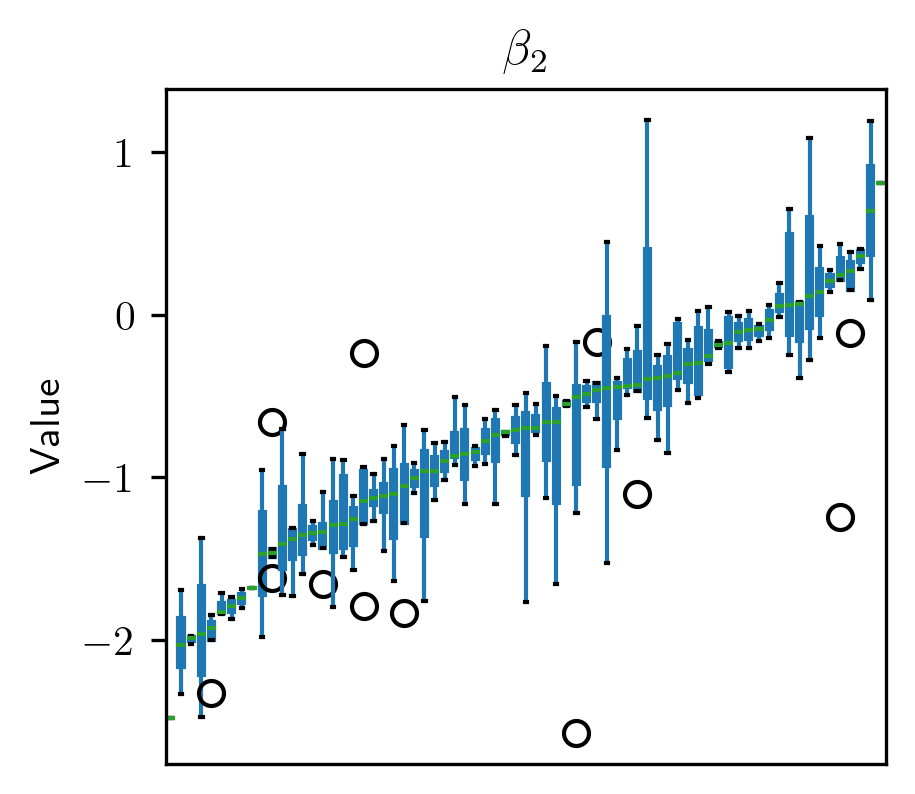
\includegraphics[width=0.3\textwidth]{files/beta_var/beta_2_var.png}
	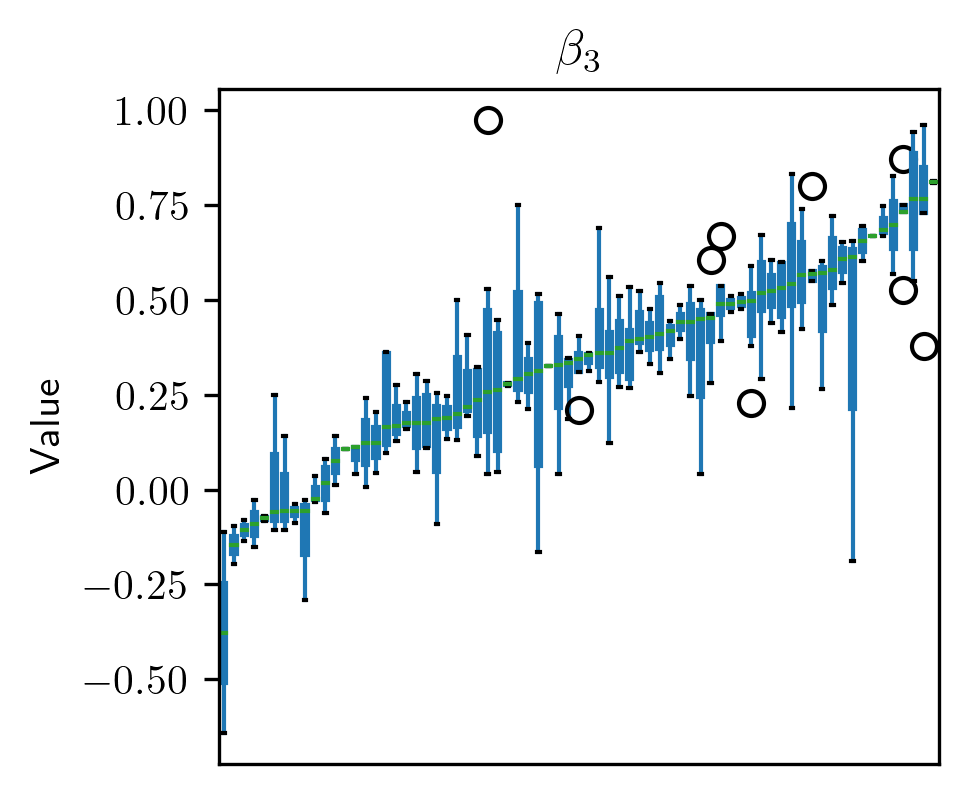
\includegraphics[width=0.3\textwidth]{files/beta_var/beta_3_var.png}
	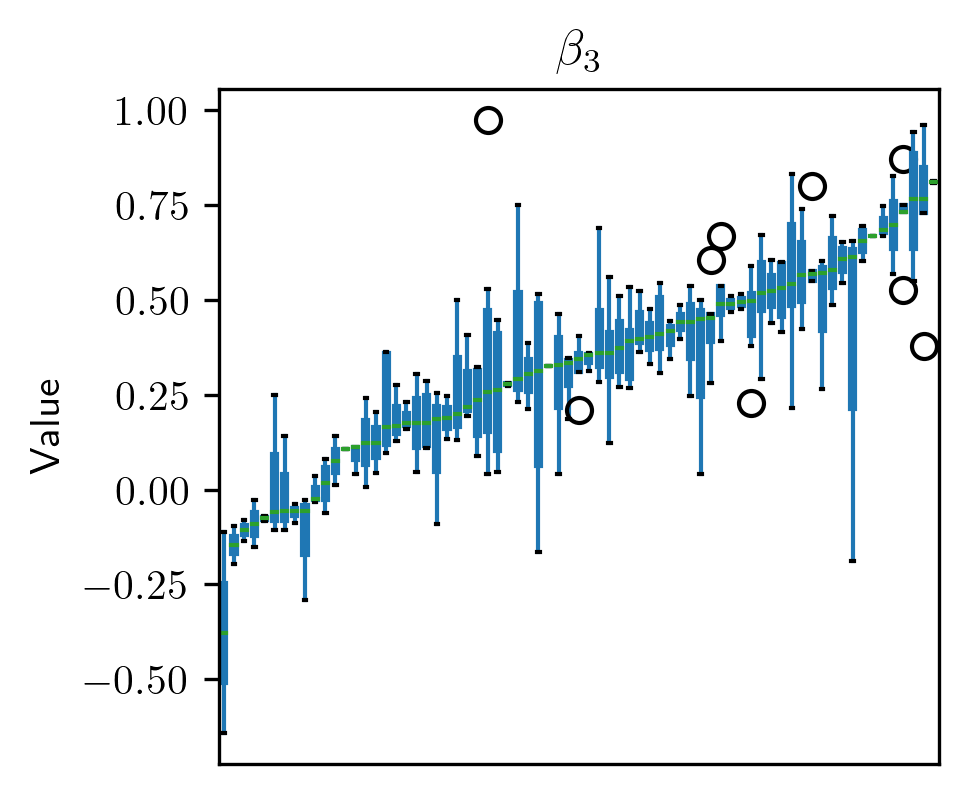
\includegraphics[width=0.3\textwidth]{files/beta_var/beta_3_var.png}
	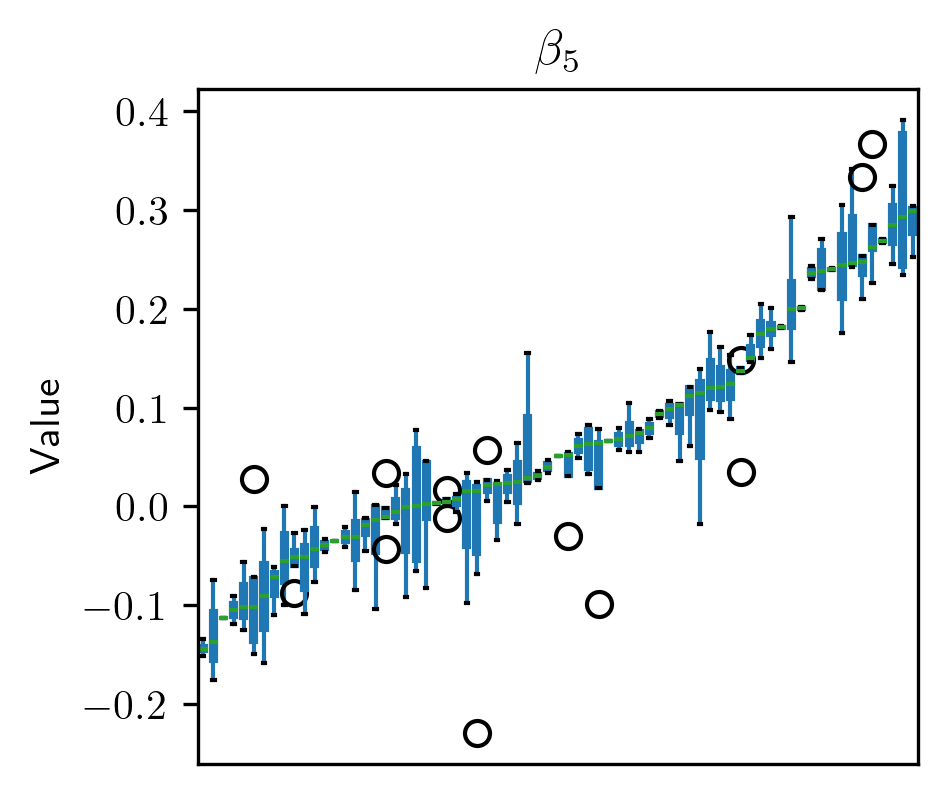
\includegraphics[width=0.3\textwidth]{files/beta_var/beta_5_var.png}
	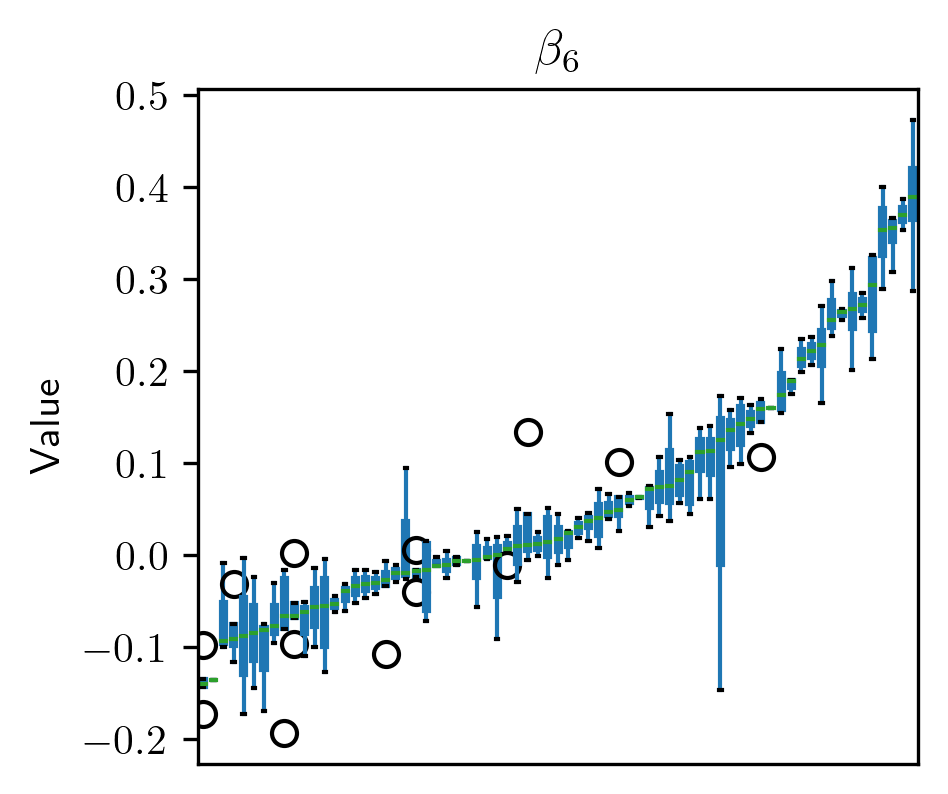
\includegraphics[width=0.3\textwidth]{files/beta_var/beta_6_var.png}
	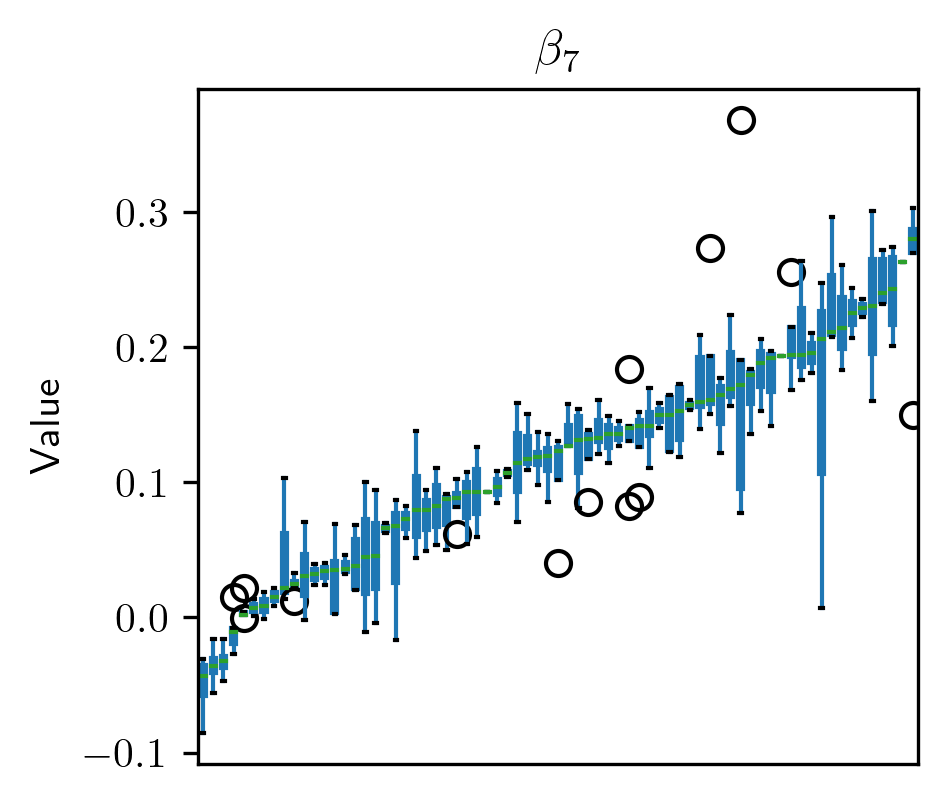
\includegraphics[width=0.3\textwidth]{files/beta_var/beta_7_var.png}
	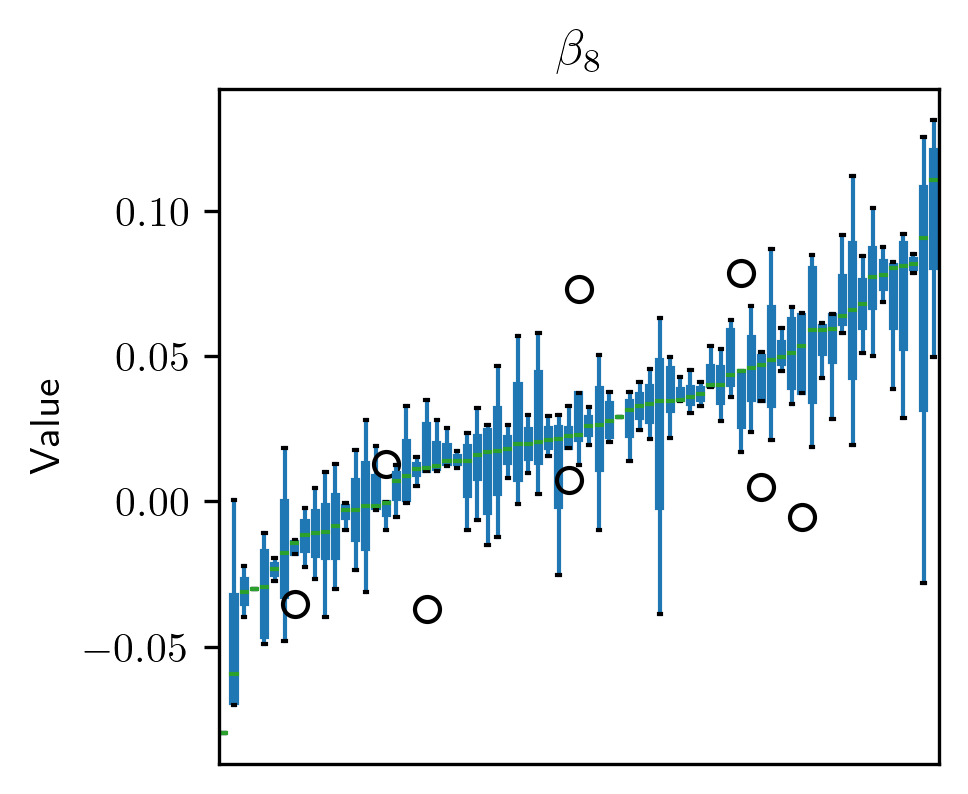
\includegraphics[width=0.3\textwidth]{files/beta_var/beta_8_var.png}
	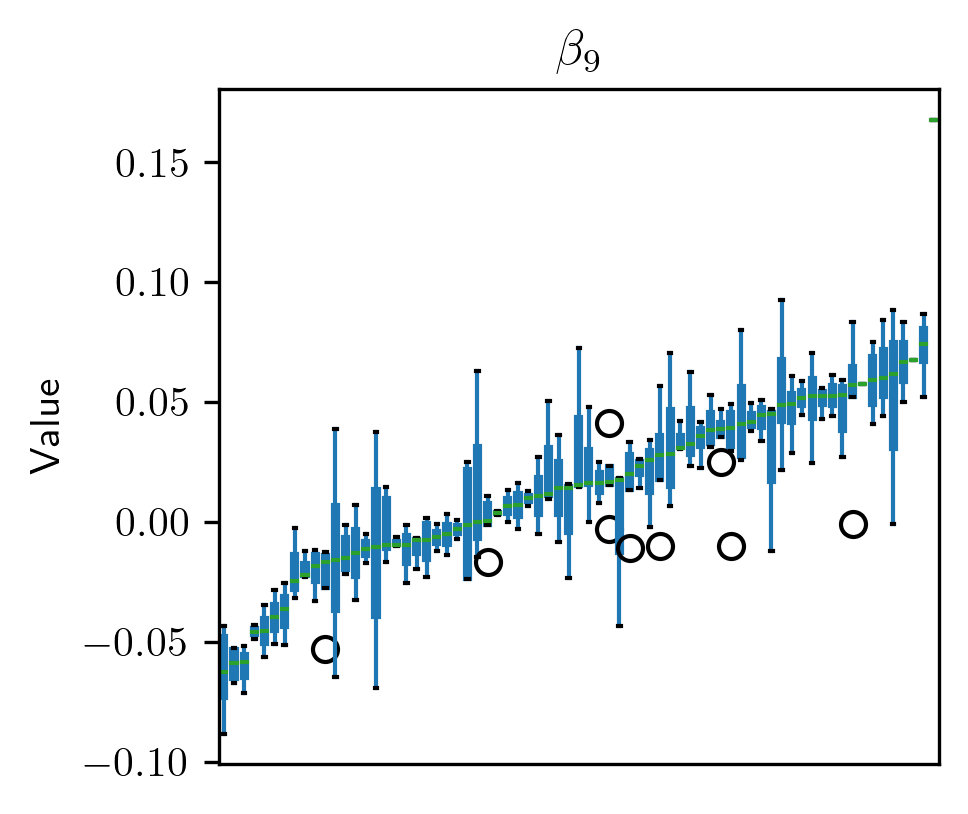
\includegraphics[width=0.3\textwidth]{files/beta_var/beta_9_var.png}
	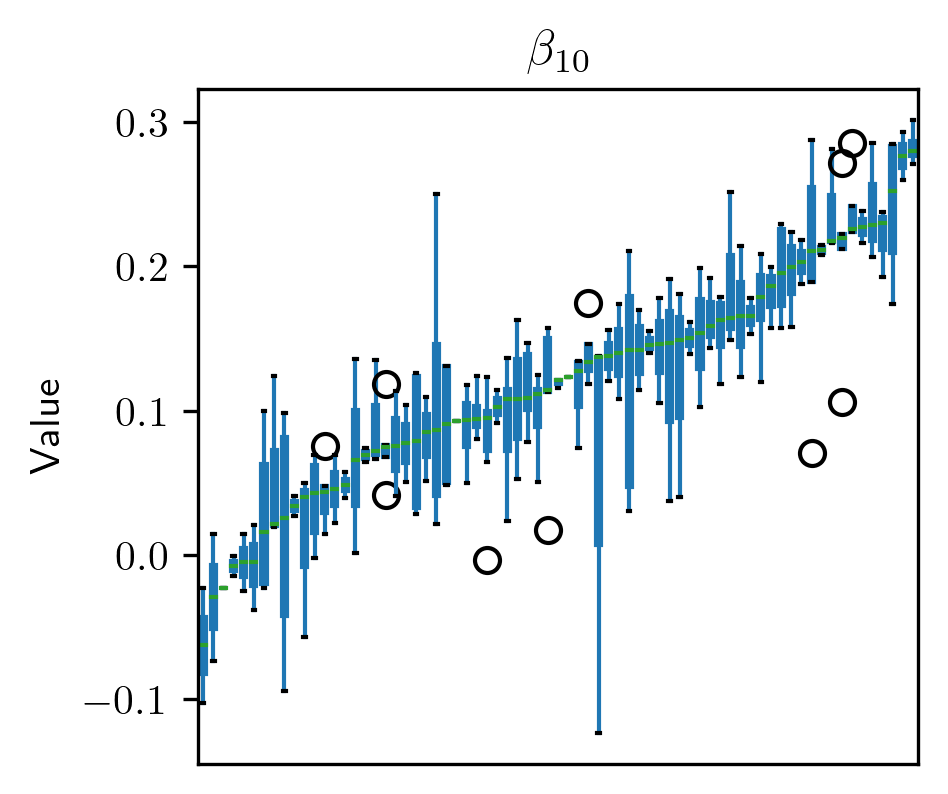
\includegraphics[width=0.3\textwidth]{files/beta_var/beta_10_var.png}

	\caption{Variation of $\beta$ per patient.}
	\label{fig:beta-var}
\end{figure}

One of the main problems of the model is that it has a lot of variance in
$\beta_1$. This parameter controls the overall height of the person (Figure
\ref{fig:beta-1-vis}). This has the effect of making the generated human bodies
vary in height, which is not desirable.

This is probably due to the fact that the training data has a lot of variance
in height, which is probably due to scanning error or our method of extracting
the \gls{smpl} parameters from the scans. Figure \ref{fig:beta-var} shows the
variation of $\beta_1$ in the dataset per patient.

To mitigate this problem, several solutions can be explored. One potential
solution is the improvement of data preprocessing, specifically in the
extraction of the SMPL parameters from the scans. By refining this process, the
quality of the training data can be significantly enhanced, reducing the
variance in the $\beta_1$ parameter and leading to more accurate predictions.

Alternatively, we could consider incorporating a form of regularization into
our model specifically targeted at controlling the variation in the height
parameter. By including a penalty term in our loss function that encourages
consistency in the height parameter, we can influence the model to maintain
more stable height predictions across sequences.

Finally, it is also possible to investigate the use of post-processing
techniques. For instance, once the model makes a prediction, we can adjust the
$\beta_1$ value based on a running average from previous sessions, thus
ensuring more consistency in the predicted height.